\chapter{Measured evidence: fresh checks and saved results}

\section{How to read evidence honestly}

Fresh checks below were run while preparing this guide on 25 November 2026. Saved database results were read from local artifacts; those database jobs were not rerun. Artifact modification dates are not embedded experiment timestamps. Historical files without a source-commit identifier cannot establish performance of this exact code revision. No live private MySQL credentials were printed or reproduced.

\section{Fresh verification of the current checkout}

\begin{longtable}{>{\raggedright\arraybackslash}p{0.258\linewidth}>{\raggedright\arraybackslash}p{0.294\linewidth}>{\raggedright\arraybackslash}p{0.368\linewidth}}
\toprule
\textbf{Check} & \textbf{Observed result} & \textbf{Interpretation} \\
\midrule
\endfirsthead
\toprule
\textbf{Check} & \textbf{Observed result} & \textbf{Interpretation} \\
\midrule
\endhead
Python 3.12 pytest, marker not db & 368 passed; 0 failures/errors; 32 deselected. Wall time reported by pytest: 104.49 s. & Current non-database tests passed. Deselected db tests are not fresh MySQL evidence. \\[4pt]
Ruff check . & All checks passed. & Static checks passed for the inspected checkout before adding these document artifacts. \\[4pt]
SQLite generated-schema self-test & 30 checks; 0 failures; seed 42; 5 shapes; up to 100 rows/table. & Checks all methods at 10 and 100 percent, replay equality and full-budget result equality. \\[4pt]
\bottomrule
\end{longtable}


\section{A saved 20-row demo: why survival and retention differ}

Source artifact: \path{results/readme-demo-1d9302050e/copy_summary.json}. Recorded UTC timestamp: 2026-11-22T06:15:03.855032+00:00. The copy retained 5 of 20 rows at a 25-percent budget, with unique PKs, zero FK violations, matching schema and a verified source read view.

\begin{longtable}{>{\raggedright\arraybackslash}p{0.129\linewidth}>{\raggedright\arraybackslash}p{0.331\linewidth}>{\raggedright\arraybackslash}p{0.184\linewidth}>{\raggedright\arraybackslash}p{0.276\linewidth}}
\toprule
\textbf{Query} & \textbf{Source / target result rows} & \textbf{Survived} & \textbf{Exact row retention} \\
\midrule
\endfirsthead
\toprule
\textbf{Query} & \textbf{Source / target result rows} & \textbf{Survived} & \textbf{Exact row retention} \\
\midrule
\endhead
Q1 & 20 / 5 & True & 25.00\% \\[4pt]
Q2 & 1 / 1 & True & 0.00\% \\[4pt]
Q3 & 20 / 5 & True & 25.00\% \\[4pt]
\bottomrule
\end{longtable}


\[\text{Average exact retention}=(0.25+0+0.25)/3=0.1667.\]

All three queries return a row set, so query survival is 100 percent. The scalar COUNT query returns one row on both sides, yet its value changes from 20 to 5, so exact result retention for that query is zero. The overall 16.67 percent is an average over queries; it is not the 25-percent physical row fraction.

\section{Historical World comparison: 18 saved runs}

Source: \path{results/raw/all_benchmark_runs.csv}. File modified UTC date: 2026-11-02. There are 18 saved successful runs: three methods, budgets 10/20/30 percent and seeds 42/123 on 5,302 source rows. This artifact predates the current source snapshot and has no runtime\_preflight column. Treat its runtime as the recorded older stage total, not a current end-to-end latency guarantee.

\begin{figure}[htbp]\centering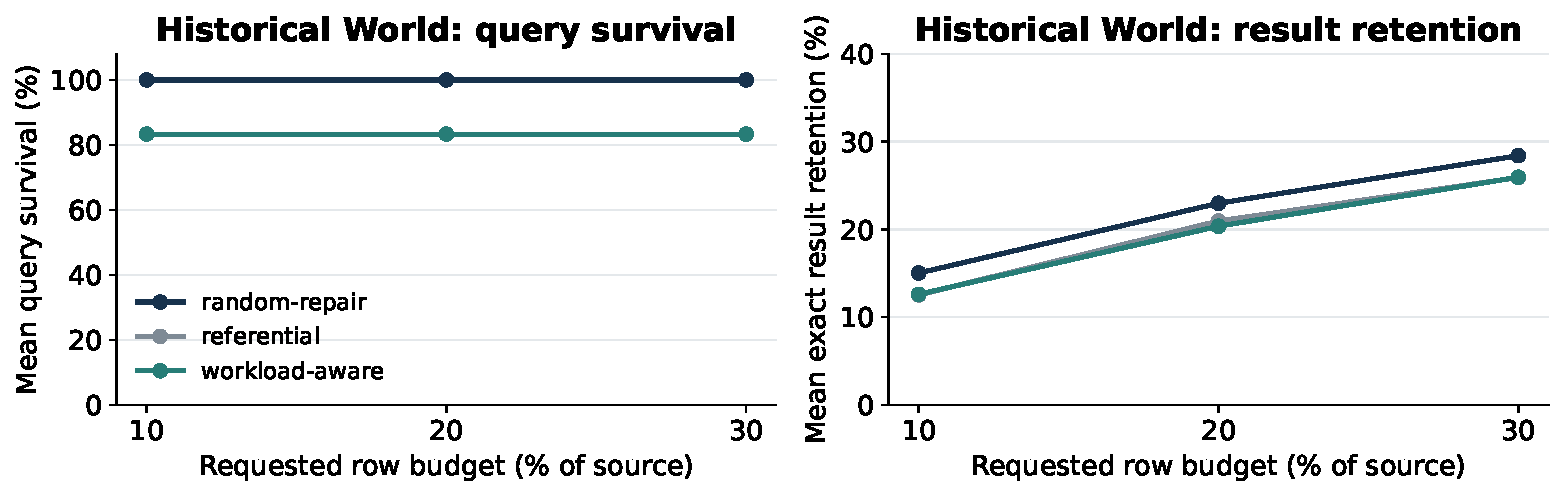
\includegraphics[width=\linewidth]{assets/historical-world.pdf}\caption{Historical World means, two seeds per method and budget. Source: local all\_benchmark\_runs.csv; artifact date 2026-11-02. These plots describe saved runs, not a new performance comparison.}\end{figure}

\begin{longtable}{>{\raggedright\arraybackslash}p{0.258\linewidth}>{\raggedright\arraybackslash}p{0.055\linewidth}>{\raggedright\arraybackslash}p{0.147\linewidth}>{\raggedright\arraybackslash}p{0.156\linewidth}>{\raggedright\arraybackslash}p{0.156\linewidth}>{\raggedright\arraybackslash}p{0.147\linewidth}}
\toprule
\textbf{Method / budget} & \textbf{n} & \textbf{Survival} & \textbf{Exact retention} & \textbf{Group metric} & \textbf{Saved time} \\
\midrule
\endfirsthead
\toprule
\textbf{Method / budget} & \textbf{n} & \textbf{Survival} & \textbf{Exact retention} & \textbf{Group metric} & \textbf{Saved time} \\
\midrule
\endhead
random-repair / 10\% & 2 & 100.00\% & 15.03\% & 47.17\% & 0.461 s \\[4pt]
random-repair / 20\% & 2 & 100.00\% & 22.98\% & 55.13\% & 0.486 s \\[4pt]
random-repair / 30\% & 2 & 100.00\% & 28.40\% & 61.74\% & 0.540 s \\[4pt]
referential / 10\% & 2 & 83.33\% & 12.53\% & 45.87\% & 0.417 s \\[4pt]
referential / 20\% & 2 & 83.33\% & 20.95\% & 53.10\% & 0.466 s \\[4pt]
referential / 30\% & 2 & 83.33\% & 25.92\% & 59.25\% & 0.546 s \\[4pt]
workload-aware / 10\% & 2 & 83.33\% & 12.60\% & 45.94\% & 0.405 s \\[4pt]
workload-aware / 20\% & 2 & 83.33\% & 20.36\% & 52.51\% & 0.495 s \\[4pt]
workload-aware / 30\% & 2 & 83.33\% & 25.95\% & 59.29\% & 0.559 s \\[4pt]
\bottomrule
\end{longtable}


In this saved artifact random-repair has higher mean survival and exact retention than workload-aware selection. This is useful evidence that the proposed heuristic is not guaranteed to win. Two seeds do not establish statistical superiority; rerun the current code with the same source/workload, broader seeds and explicit acceptance before making comparative claims.

\section{Saved MySQL synthetic scale evidence}

Source: \path{results/scale/6893236af2c9/evidence.json}. State: completed; backend: MySQL; Python: 3.10.11. This recorded run covers 5 shapes and 30 checks per scale sample. The requested row scale is a per-table generation bound, not a total-database row count.

\begin{longtable}{>{\raggedright\arraybackslash}p{0.138\linewidth}>{\raggedright\arraybackslash}p{0.322\linewidth}>{\raggedright\arraybackslash}p{0.138\linewidth}>{\raggedright\arraybackslash}p{0.175\linewidth}>{\raggedright\arraybackslash}p{0.147\linewidth}}
\toprule
\textbf{Rows/table bound} & \textbf{Actual source totals by case} & \textbf{Checks / failures} & \textbf{Wall / CPU time} & \textbf{Peak client RSS} \\
\midrule
\endfirsthead
\toprule
\textbf{Rows/table bound} & \textbf{Actual source totals by case} & \textbf{Checks / failures} & \textbf{Wall / CPU time} & \textbf{Peak client RSS} \\
\midrule
\endhead
1000 & 1,446, 1,930, 3,558, 2,794, 1,051 & 30 / 0 & 73.93 / 50.42 s & 174.69 MiB \\[4pt]
10000 & 15,649, 17,077, 40,463, 31,236, 12,321 & 30 / 0 & 426.58 / 342.59 s & 262.73 MiB \\[4pt]
\bottomrule
\end{longtable}


The largest recorded case here has 40,463 total source rows and a sampled client-process peak of about 262.73 MiB for its scale sample. The measure excludes MySQL server resource use and is a sampled process peak, not a continuous exact maximum. It is explicitly synthetic evidence with production\_certification=False.

\section{What has not been established}

The project does not contain a current production-capacity certification, a guarantee that every database in the download list has been sliced end to end, a universal method winner, or a classification F1/FN evaluation. A 5,000,000-row resource policy is a configurable guard, not evidence of a successful five-million-row benchmark. The sanitized evidence snapshot and source hashes accompany this guide so each reported value remains traceable.